\documentclass{sciposter}
\usepackage{lipsum}
\usepackage{epsfig}
\usepackage{amsmath}
\usepackage{amssymb}
\usepackage{multicol}
\usepackage{graphicx,url}
\usepackage[T1]{fontenc}
\usepackage[table]{xcolor}
\usepackage[utf8]{inputenc}
\newtheorem{Def}{Definition}


\title{Performance Impact of Exploiting Undefined Behavior in C/C++}
\author{*Lucian I. Popescu, **Nuno P. Lopes}

\institute 
{
*Faculty of Automatic Control and Computer Science,\\
Politehnica University of Bucharest \\
** Instituto Superior Técnico, \\
Universidade de Lisboa
}

\email{*lucian.popescu187@gmail.com, **nuno.lopes@tecnico.ulisboa.pt}

% TODO: change them with higher resolution logos
\rightlogo[1]{logo-upb}
\leftlogo[1]{logo-ist}


\begin{document}

\conference{{\bf EuroLLVM 23}, 11th May 2023, Glasgow, GB}

%\LEFTSIDEfootlogo  
% Uncomment to put footer logo on left side, and 
% conference name on right side of footer

% Some examples of caption control (remove % to check result)

%\renewcommand{\algorithmname}{Algoritme} % for Dutch

%\renewcommand{\mastercapstartstyle}[1]{\textit{\textbf{#1}}}
%\renewcommand{\algcapstartstyle}[1]{\textsc{\textbf{#1}}}
%\renewcommand{\algcapbodystyle}{\bfseries}
%\renewcommand{\thealgorithm}{\Roman{algorithm}}

\maketitle

\begin{multicols}{3}

\section{Introduction}
Clang and LLVM use undefined behavior (UB) to issue code optimizations.
Currently, there is no study that evaluates the performance impact of this class
of optimizations. We fill this gap by presenting some early results in this
area. Phoronix Test Suite was used to evaluate the performance of a diverse set
of applications, including webservers, compression algorithms, graphical
environments, etc. By compiling each application with flags that trigger
specific UBs, we gathered various metrics (requests per second, MB/s, FPS,
etc) for further analysis.

\begin{large}
Early results show that in nearly 90\% of the cases
the performance impact is insignificant (between -2\% and 2\%).
\end{large}

\section{Experiment Setup}
The performance tests were run on a machine with the following specs:
\begin{itemize}
\item Processor: 2 x Intel Xeon E5-2680 v2 @ 3.60GHz (20 Cores / 40 Threads), MicroArch: IvyBridge
\item OS: Debian 11, kernel: 5.10.0-21-amd64 (x86\_64)
\item Compiler: Clang 15.0.7
\end{itemize}
\bigbreak
\bigbreak
The experiments were conducted using the following steps:
\begin{itemize}
\item Compile the benchmark with no UB flags enabled (baseline)
\item Compile the benchmark using one UB flag at a time
\item Run baseline using Phoronix and fetch the results
\item Run the benchmarks with UB flags using Phoronix and fetch the results
\item Compare the UB flags benchmark results with the baseline
\end{itemize}

\section{Undefined Behavior Flags}

% TODO: make the second column syntactically parallel
\rowcolors{2}{gray!25}{white}
\begin{tabular}{p{8cm}|p{15cm}|}
\rowcolor{gray!50}
Flag name & Flag Description\\
Existing Flags & \\
-fwrapv & Treat signed integer overflow as two's complement. Drops `nsw' from IR.\\
-fno-strict-aliasing & Don't use type-based alias analysis. Drops `!tbaa' from IR. \\
-fstrict-enums & Enable optimizations that take advantage of enum's value ranges. Adds `!range' from IR.\\
-fno-delete-null-pointer-checks & Assume that programs can safely dereference null pointers. \\
-fno-finite-loops & Don’t assume that all loops are finite. `!mustprogress' is not added to any loop or function.\\
Flags Added by Us & \\
-fconstrain-shift-value & Mask shift RHS so it doesn't produce poison when RHS >= bitwidth. \\
-fno-constrain-bool-value & Do not constrain bool values in \{0,1\}. Drops `!range' from IR.\\
-fno-use-default-alignment & Use alignment of 1 for all memory operations including load, store, memcpy, etc. Global variables and alloca's remain unaffected.\\
TODO Flags & \\
& Change uninitialized loads from undef to zero . \\
& Don't treat out-of-bounds memory accesses as UB. \\
& Don't treat use-after-free accesses as UB.\\
& Don't use object-based rules in alias analysis (use an aassembly-like memory mode). \\
& Remove arithmetic-related UBs (division by 0, etc). \\
\end{tabular} \\

\textbf{\textit{-fwrapv}} \\
Out of 162 data points, 83\% values are in the interval of \( [-2,\;2] \), 
6\% exhibit positive performance impact and 11\% exhibit negative
performance impact. This flag has the biggest overall negative 
performance impact, as presented in Figure~\ref{fig:espeak}.

\begin{figure}[h!]
\centering
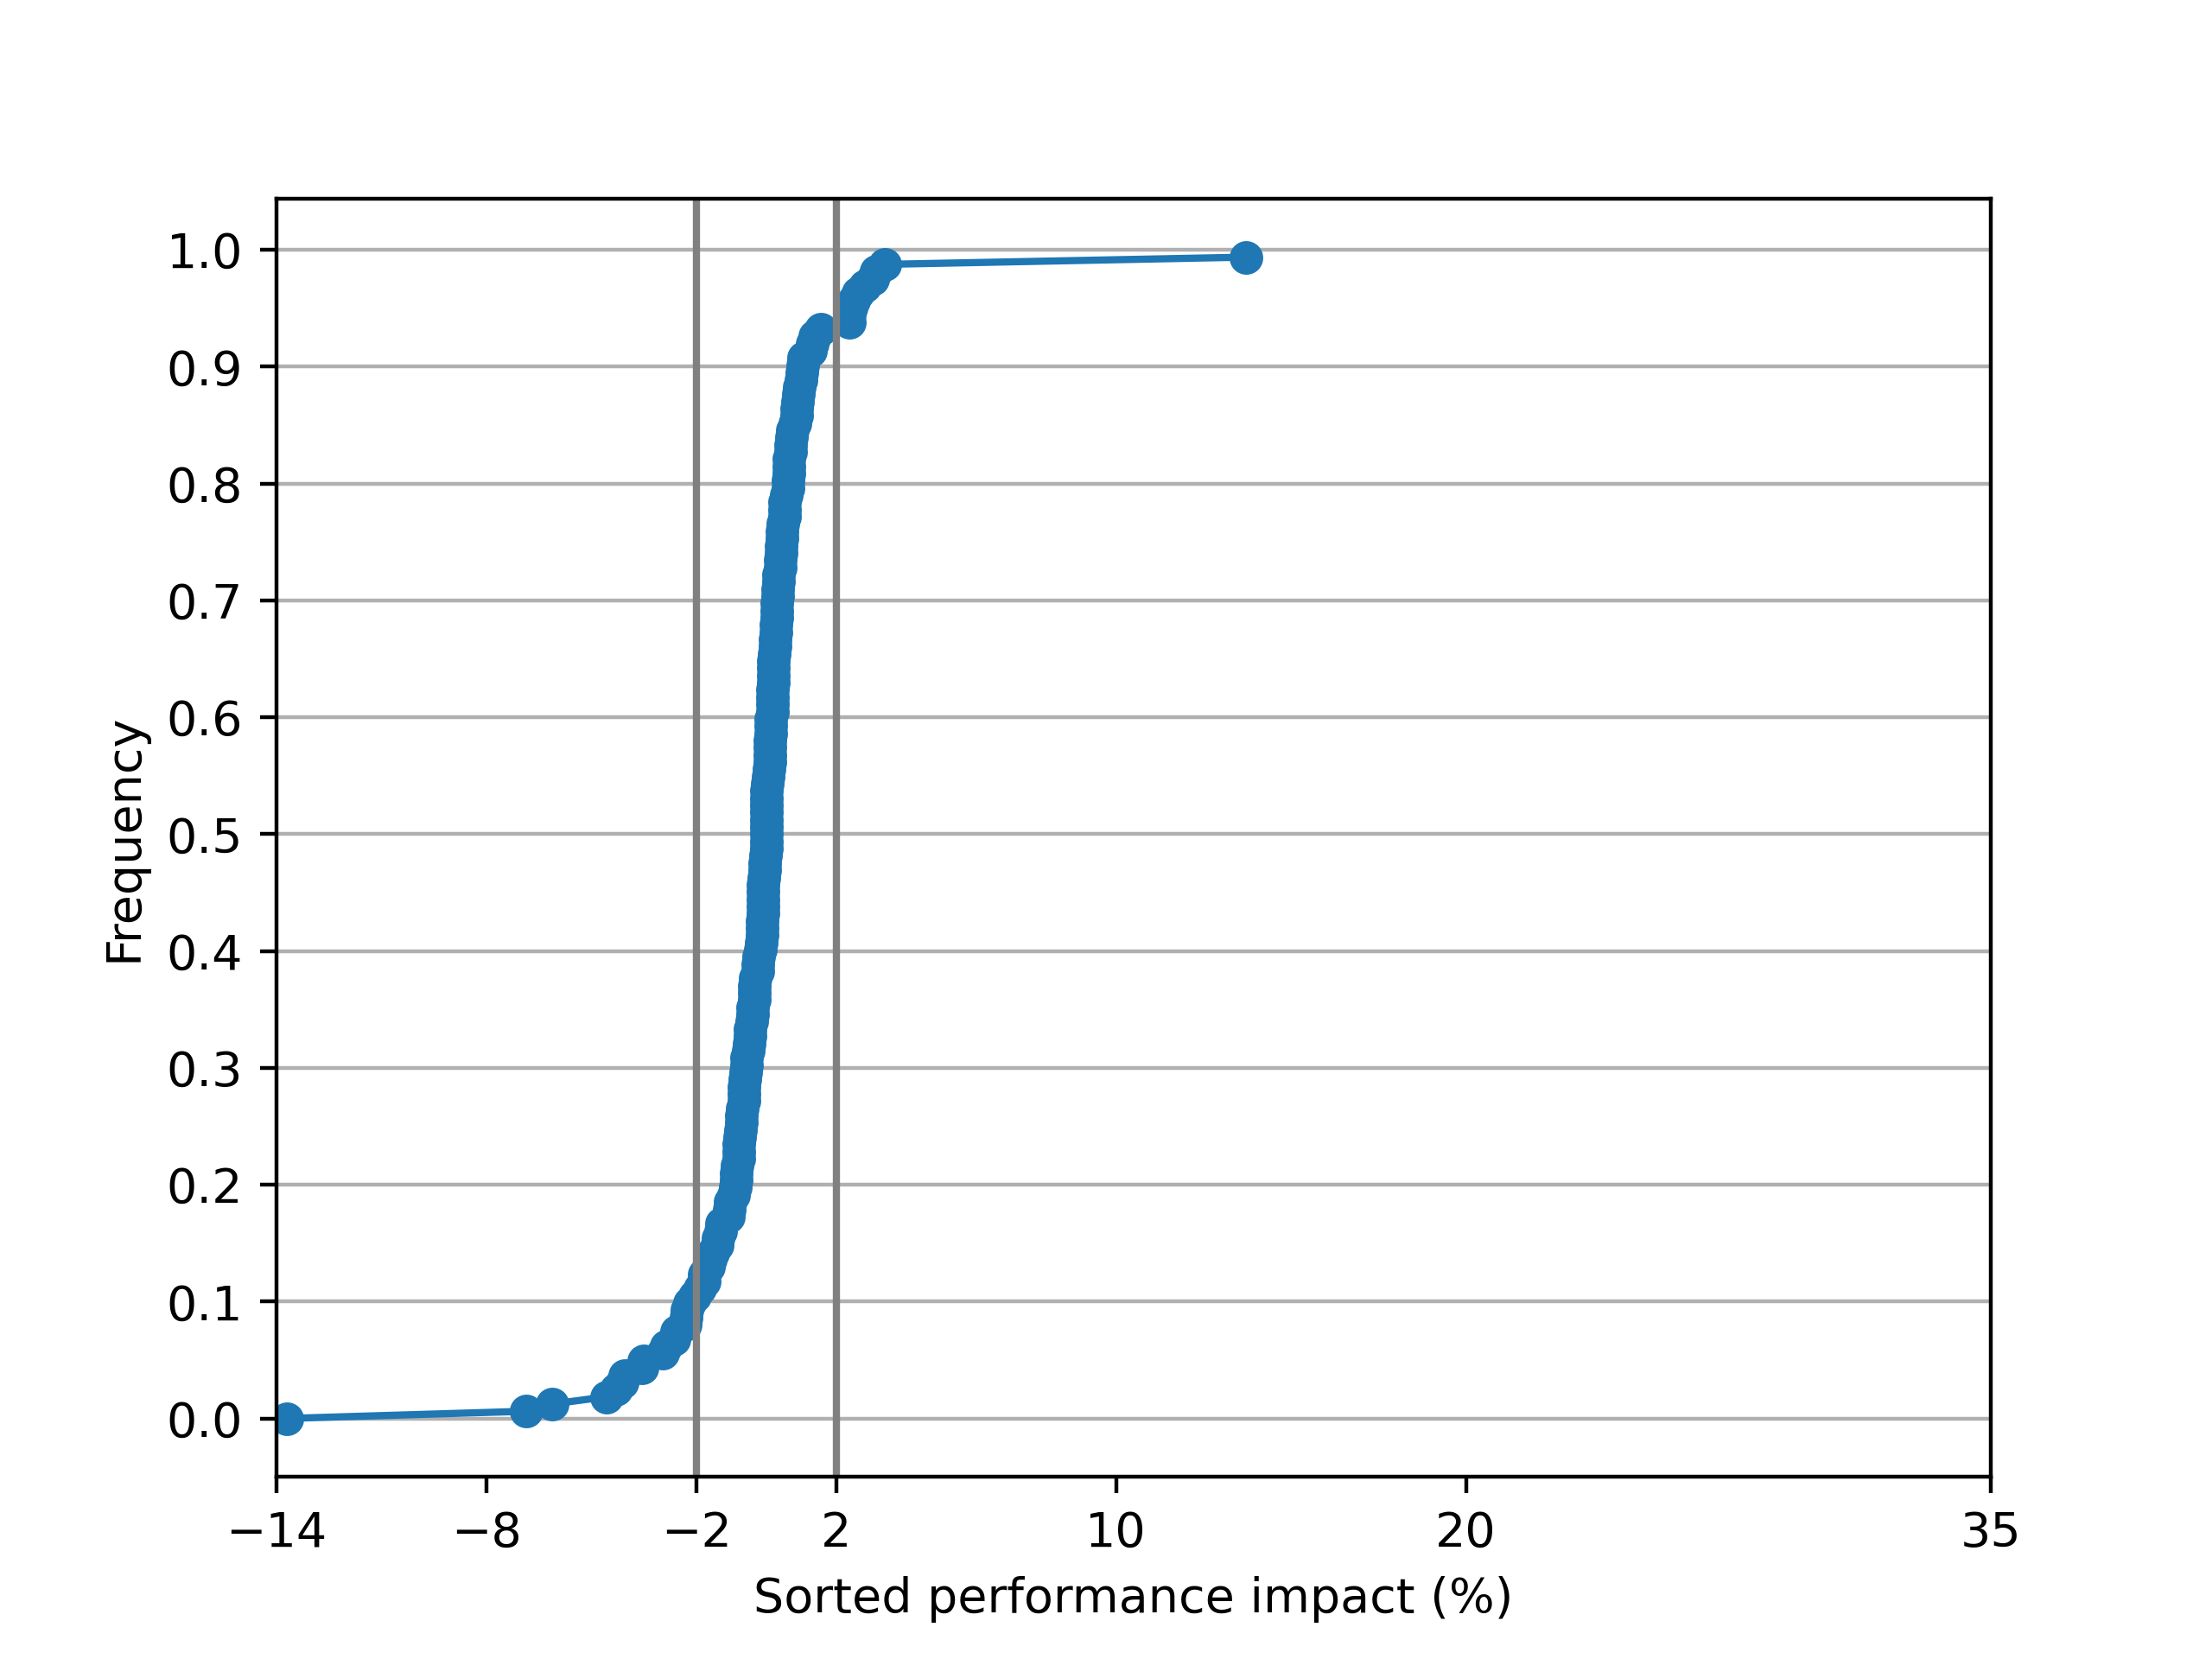
\includegraphics[scale=1.2]{fwrapv}
\caption{CDF of performance impact for -fwrapv}
\end{figure}

Other benchmarks with negative impact: FFTW - Float + SSE - Size: 1D FFT Size
256, uvg266 (Video Encoder). Other benchmarks with positive impact: OpenSSL -
RSA4096.

\begin{figure}[h!]
\centering
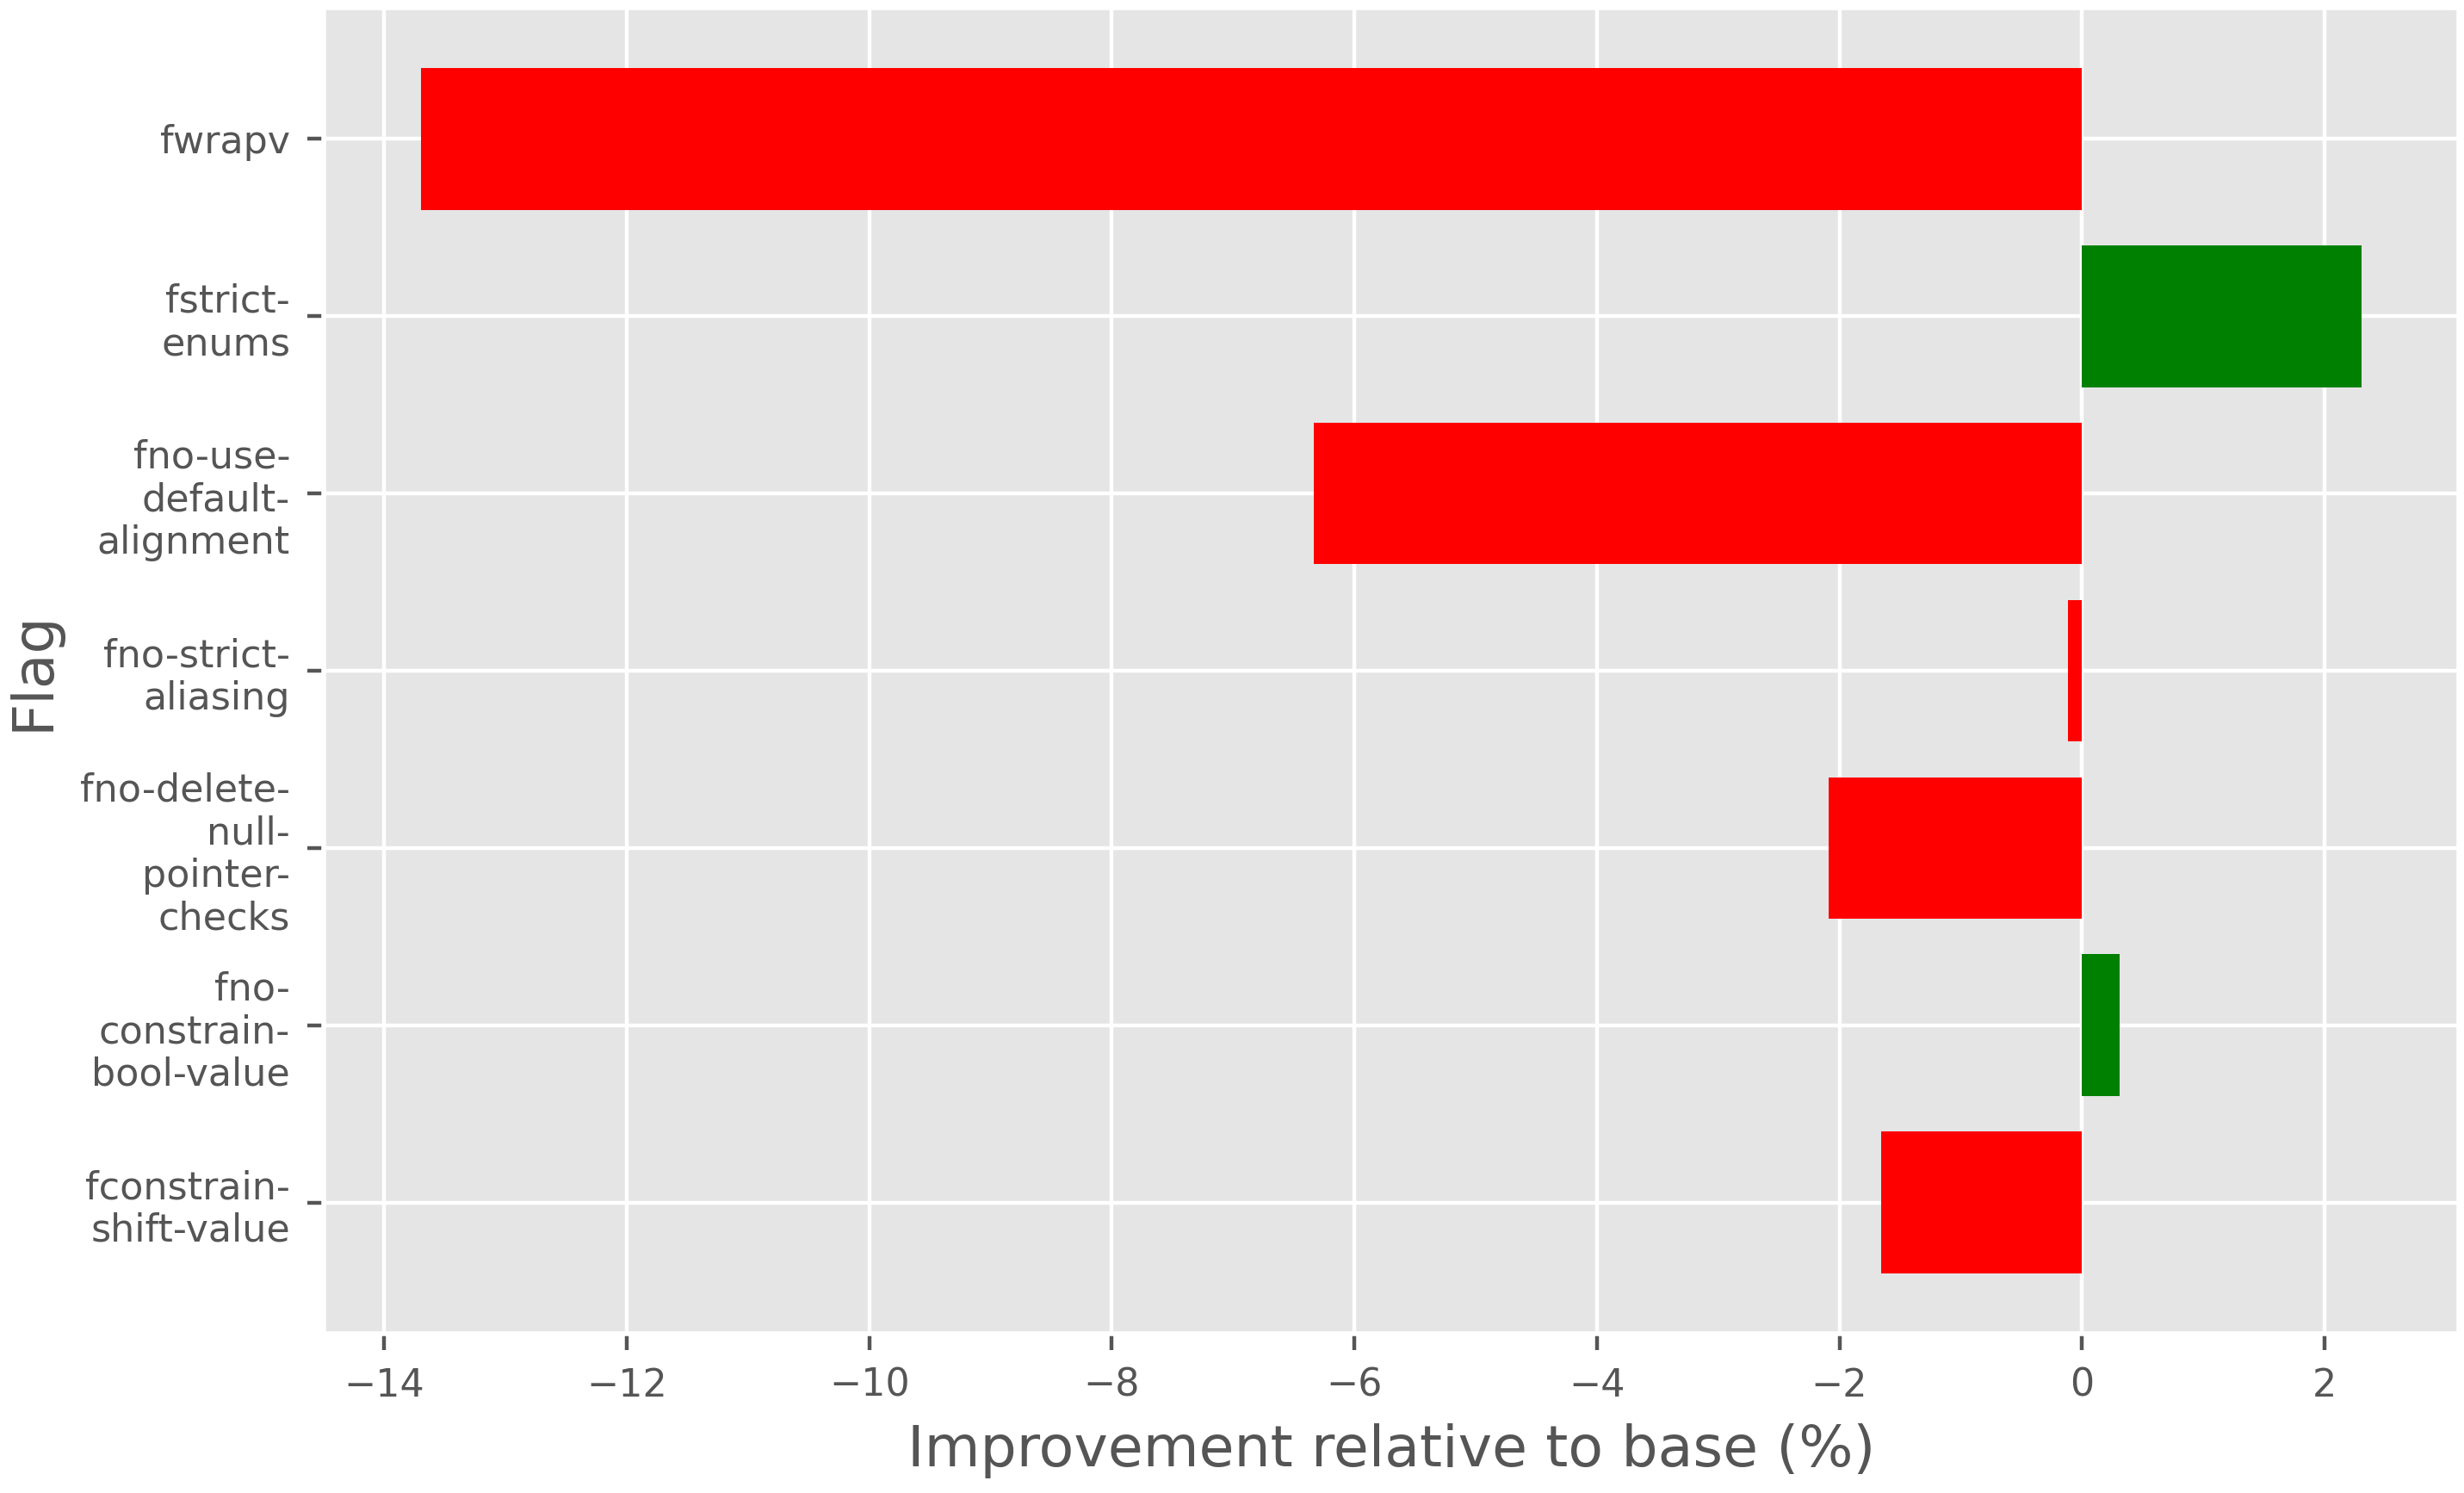
\includegraphics[scale=1.2]{espeak} \\
\caption{eSpeak-NG Speech Engine - Text-To-Speech Synthesis, Baseline:
41.59 Sec} 
\label{fig:espeak}
\end{figure}

\textbf{\textit{-fno-strict-aliasing}} \\
Out of 162 data points, 88.8\% values are in the interval of \( [-2,\;2] \), 
3\% exhibit positive performance impact and 8.2\% exhibit negative
performance impact. This is the most balanced flag up until this moment.

\begin{figure}[h!]
\centering
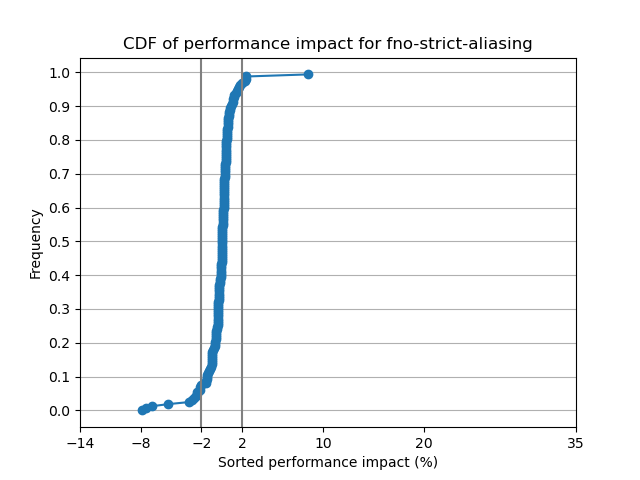
\includegraphics[scale=1.2]{fno-strict-aliasing}
\caption{CDF of performance impact for fno-strict-aliasing}
\end{figure}

\textbf{\textit{-fconstrain-shift-value}} \\
Out of 161 data points, 88.8\% values are in the interval of \( [-2,\;2] \), 
8.1\% exhibit positive performance impact and 3.1\% exhibit negative
performance impact. This flag has the biggest overall positive 
performance impact, as presented in Figure~\ref{fig:gtkperf}.

\begin{figure}[h!]
\centering
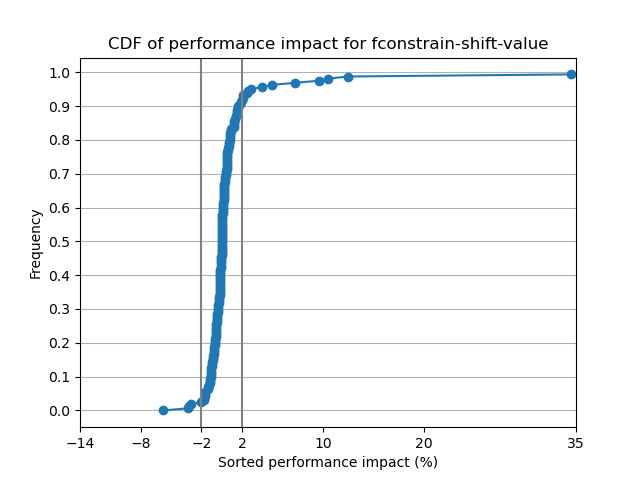
\includegraphics[scale=1.2]{fconstrain-shift-value}
\caption{CDF of performance impact for -fconstrain-shift-value}
\end{figure}

Other benchmarks with negative impact: GraphicsMagick - Operation: Swirl, PJSIP
- Method: OPTIONS Stateful. Other benchmarks with positive impact: OpenSSL -
AES-256-GCM.

\begin{figure}[h!]
\centering
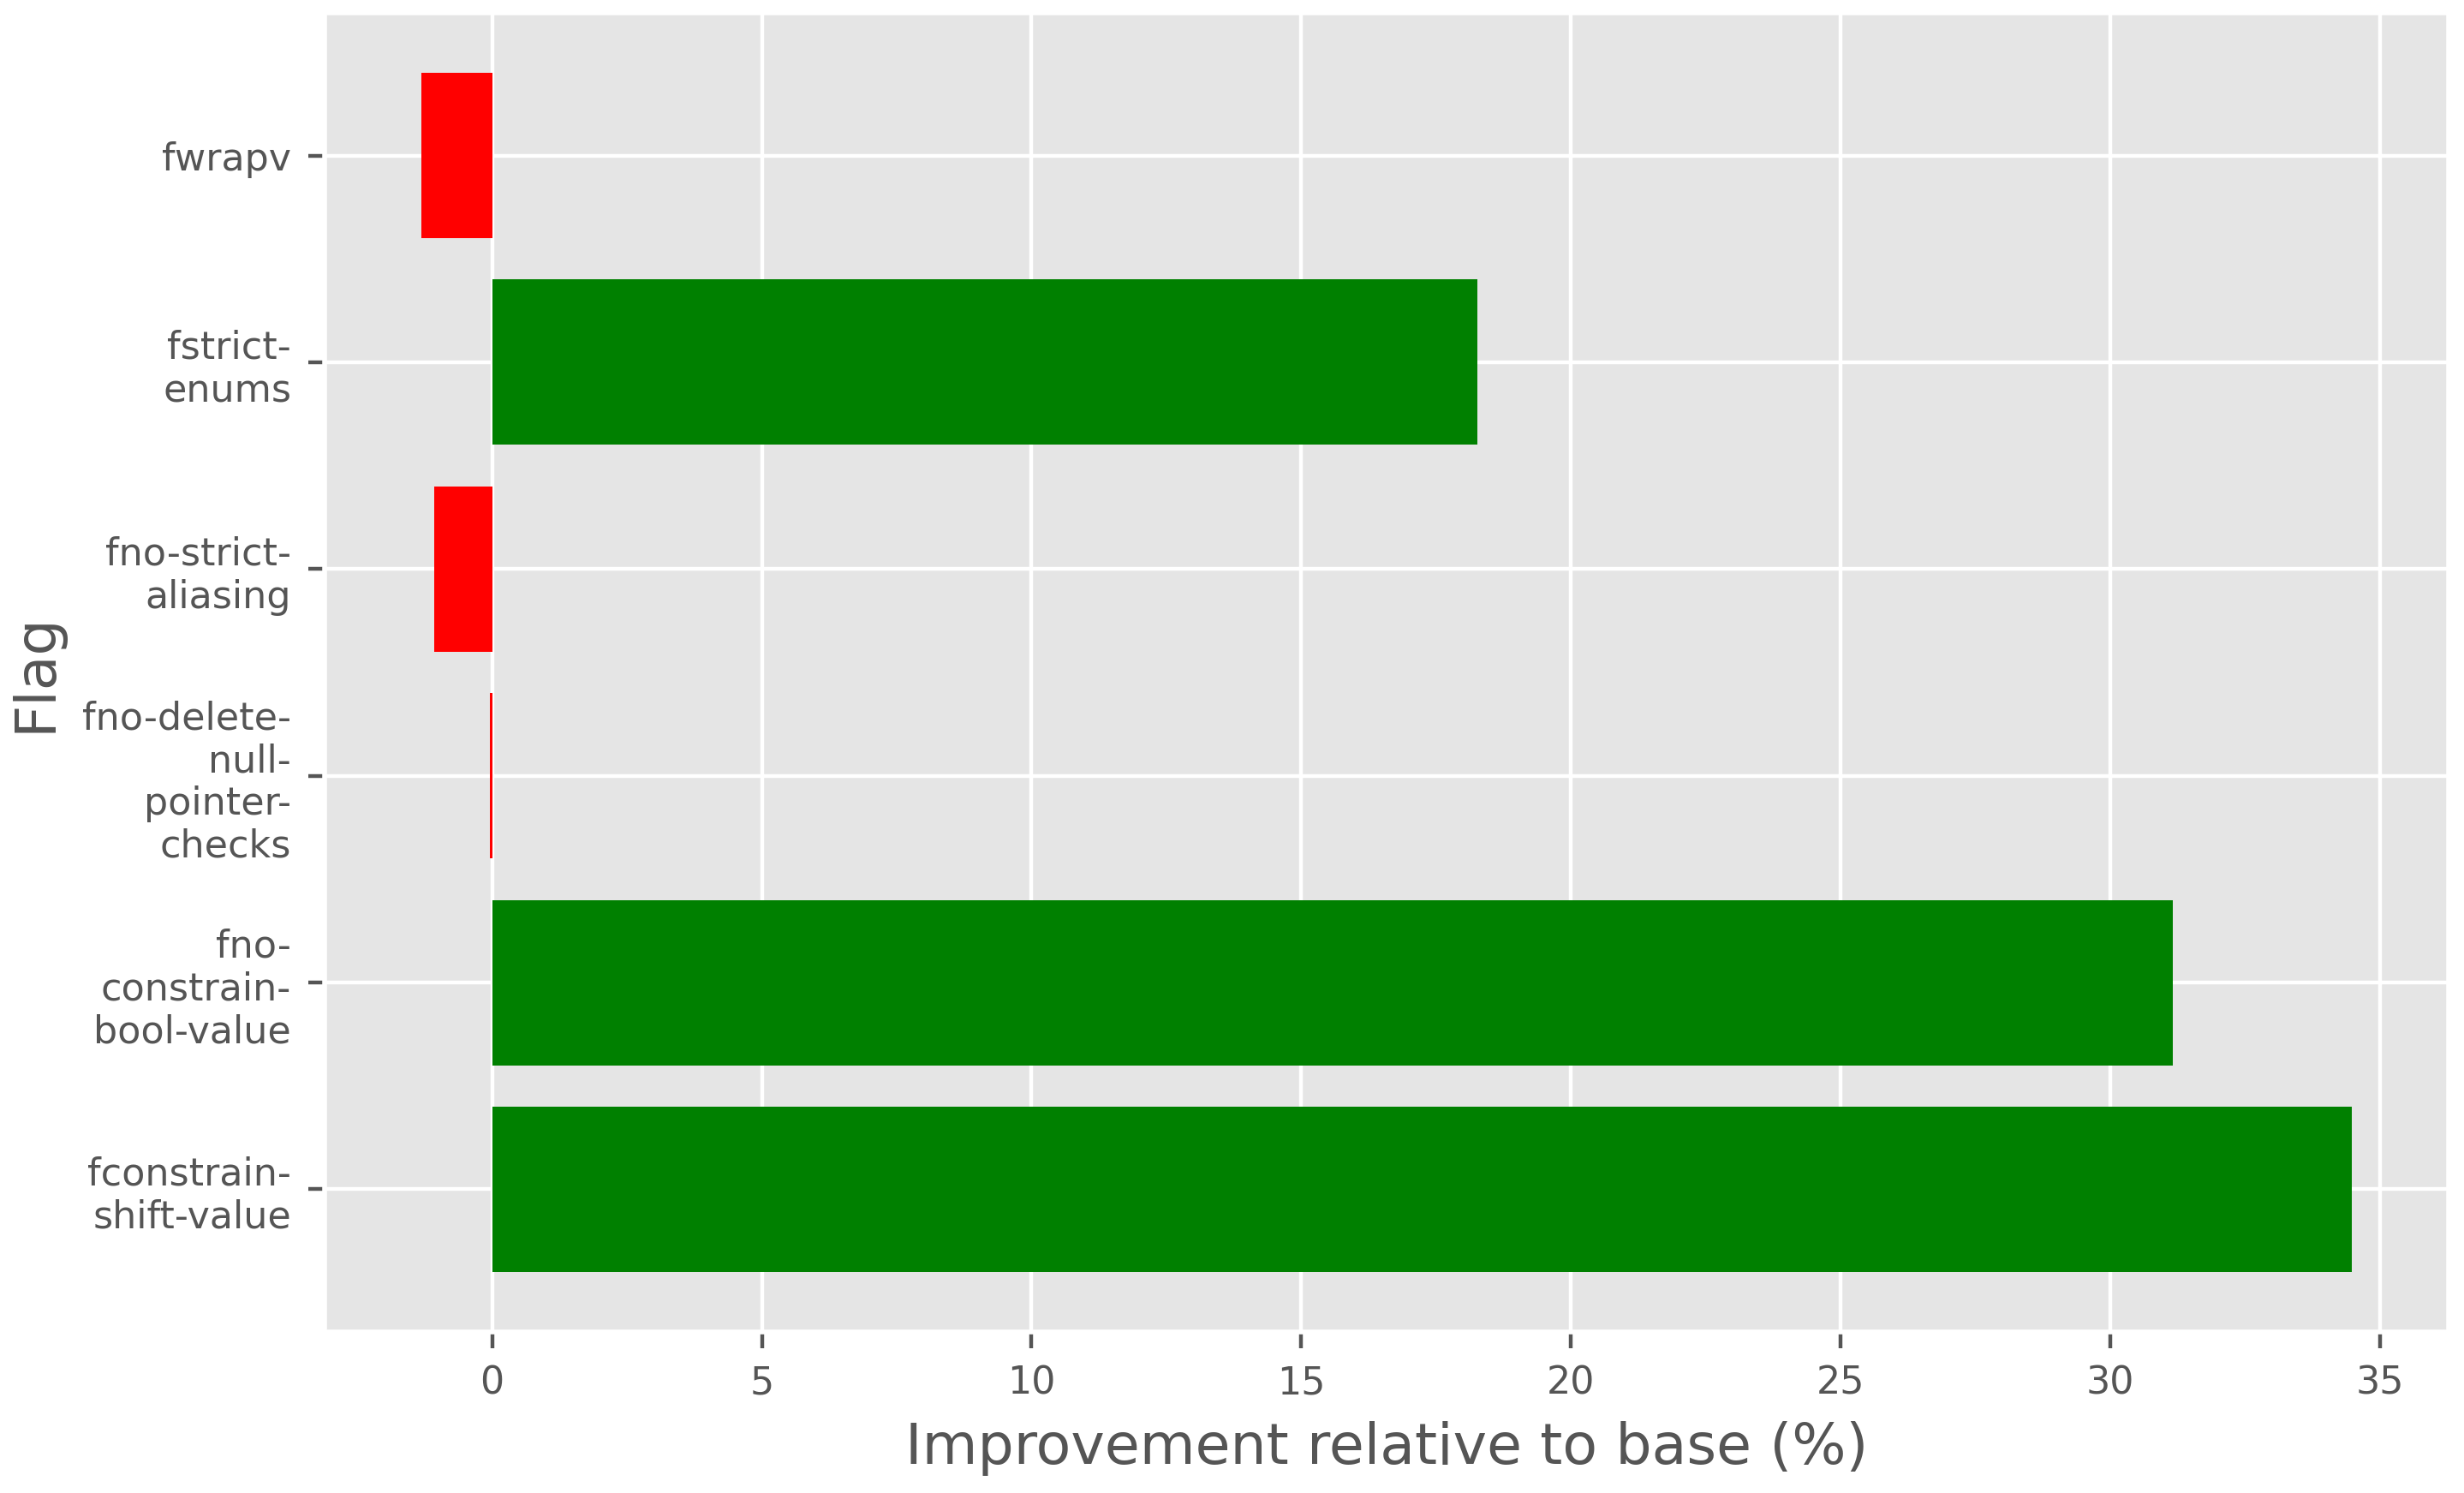
\includegraphics[scale=1.3]{gtkperf} \\
\caption{GtkPerf - GTK Widget: GtkDrawingArea - Pixbufs, Baseline: 170.08 Sec}
\label{fig:gtkperf}
\end{figure}

\textbf{\textit{-fno-use-default-alignment}} \\
Out of 158 data points, 85.5\% values are in the interval of \( [-2,\;2] \), 
10.5\% exhibit positive performance impact and 4\% exhibit negative
performance impact. For this flag we expected the negative impact to be greater
than the positive impact.

\begin{figure}[h!]
\centering
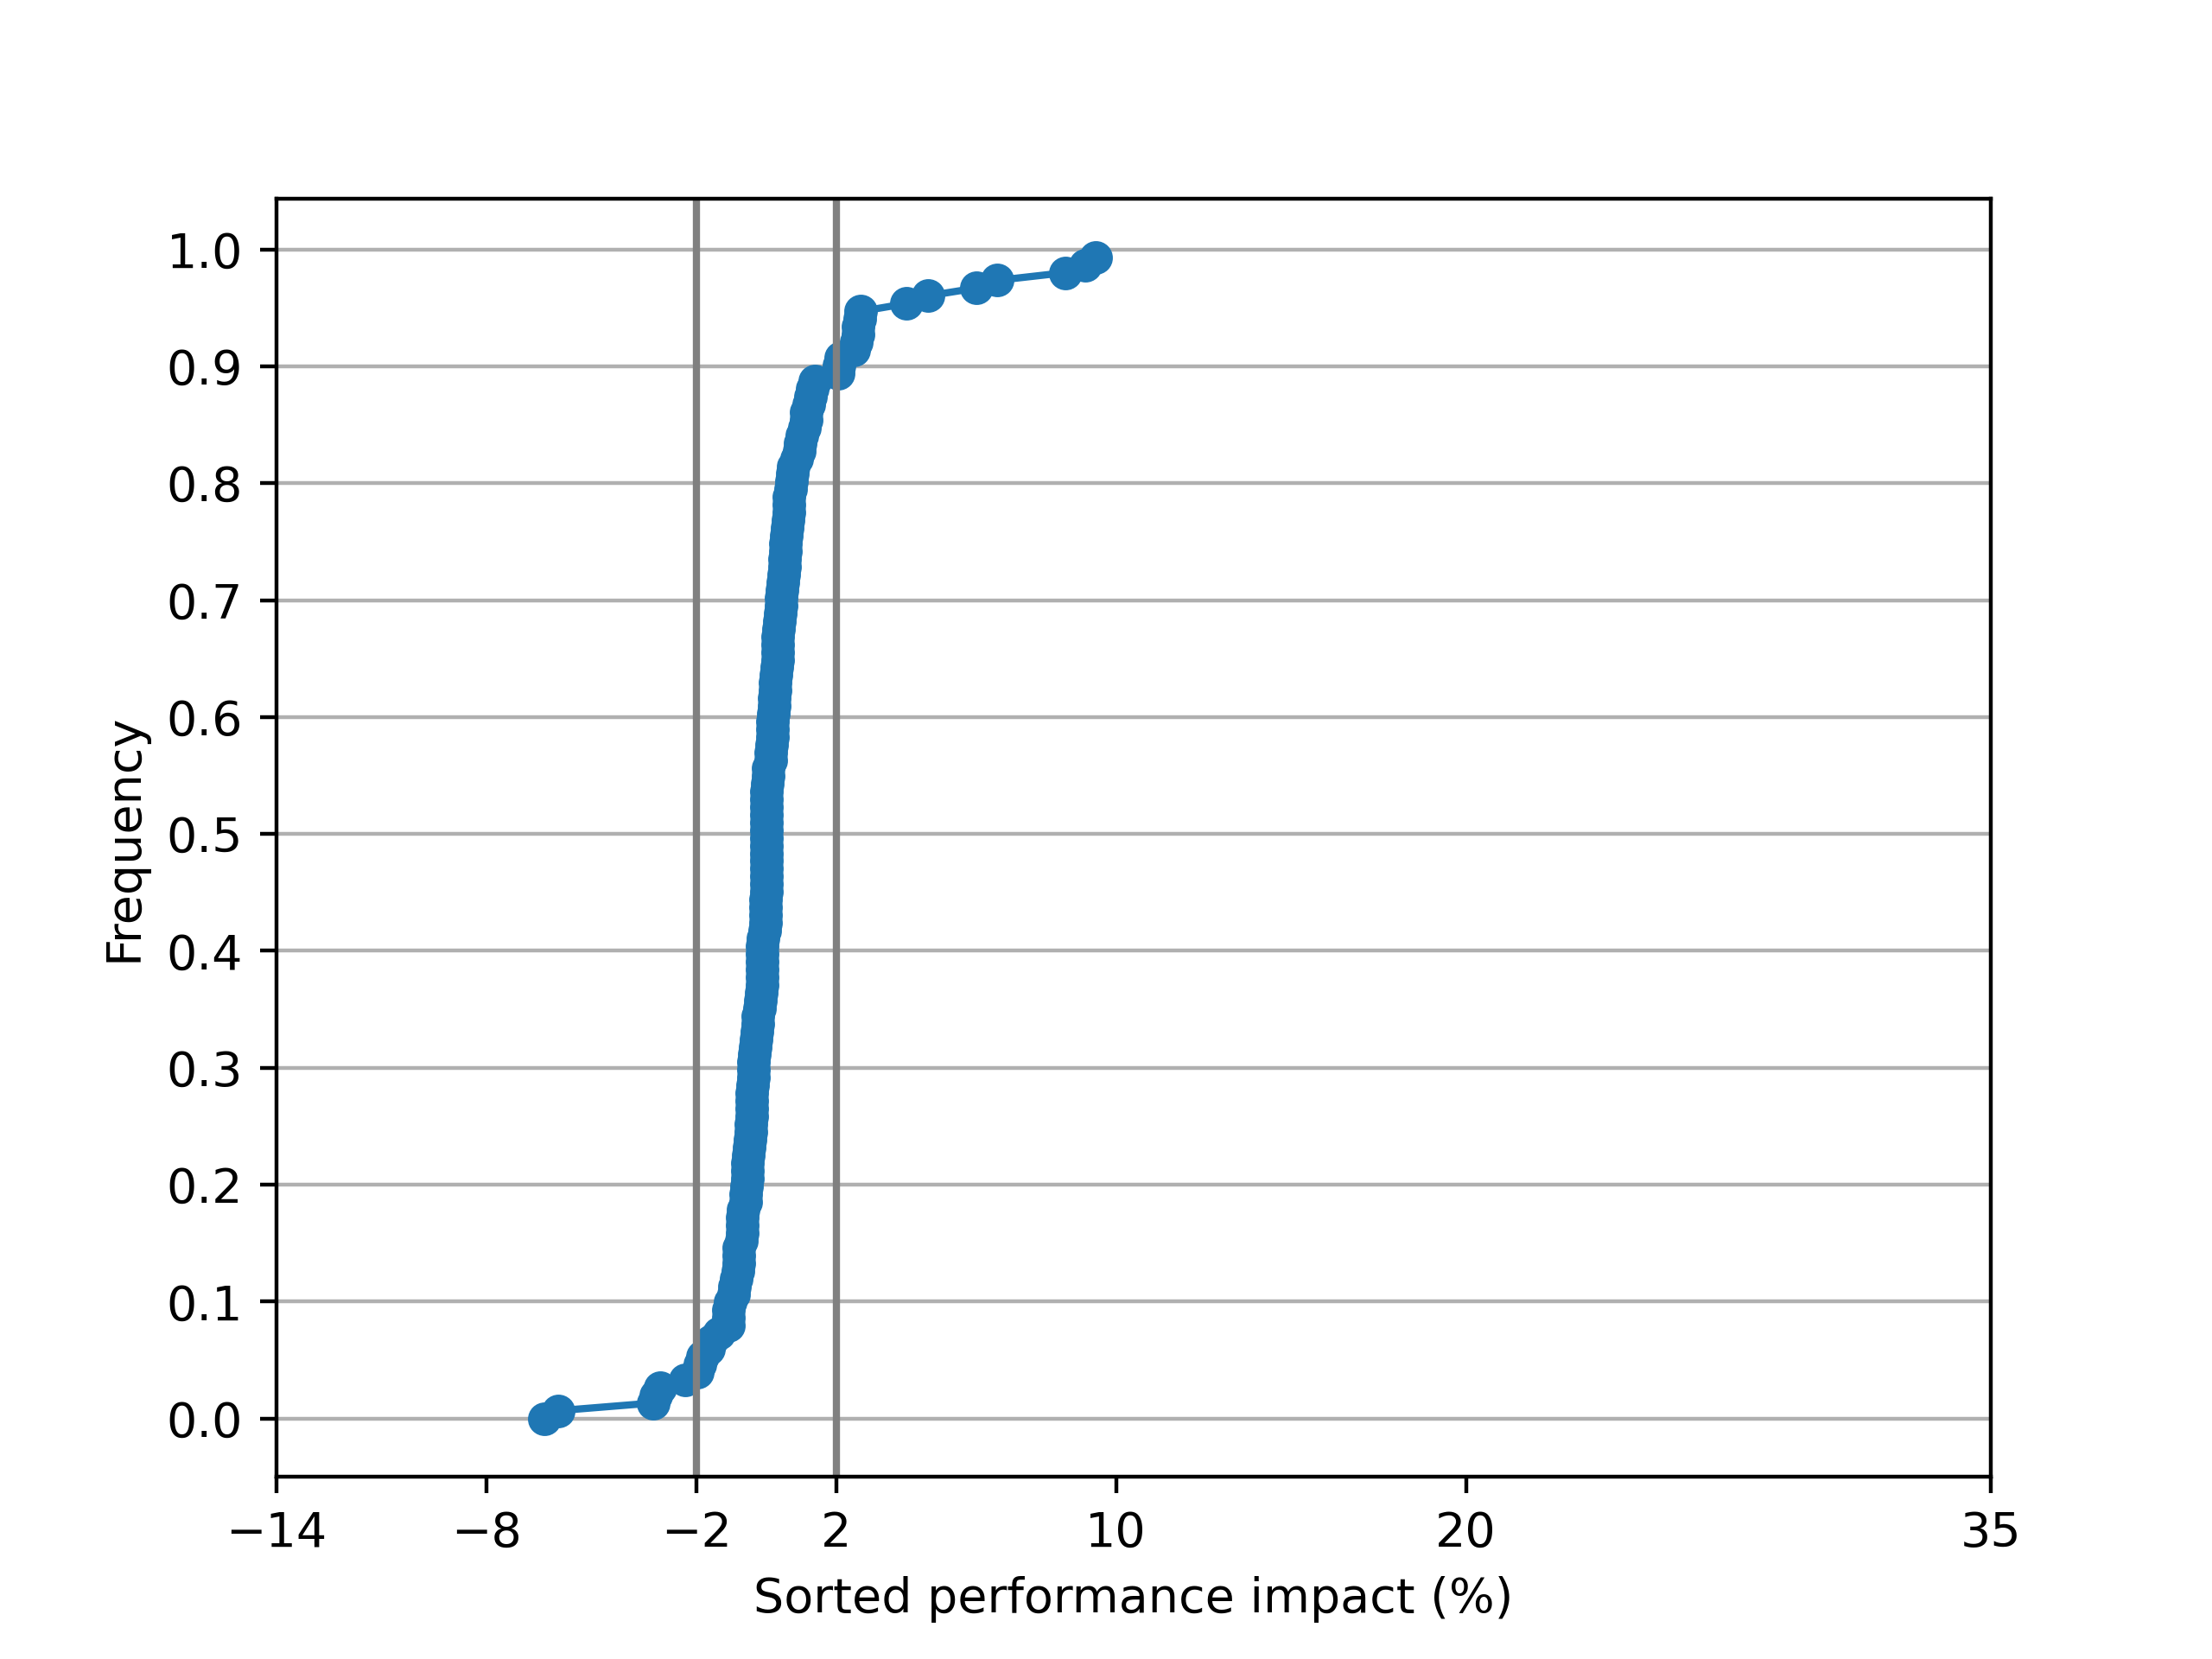
\includegraphics[scale=1.2]{fno-use-default-alignment}
\caption{CDF of performance impact for -fno-use-default-alignment}
\end{figure}

\section{Future work}
\begin{itemize}
\item Implement and benchmark other classes of UB.
\item Run the benchmarks on different hardware architectures (AMD, ARM).
\item Find a method of discovering new UBs (maybe using Alive2).
\item Run the benchmarks taking into account LTO and PGO.
\end{itemize}

%%% References

%% Note: use of BibTeX als works!!
\end{multicols}

\end{document}

% TODOS:
% mention that this is not a sanitizer
